\documentclass{article}
\usepackage[margin=1in]{geometry}
\usepackage{amsmath,amsfonts,amssymb}
\usepackage{listings}
\usepackage{color}
\usepackage{graphicx}
\usepackage{subfig}
\usepackage{blkarray}
\usepackage{multirow}
\usepackage{float}
\usepackage{caption}
\usepackage{subcaption}
\begin{document}
\begin{titlepage}
	\setlength{\parindent}{0pt}
	\large

\vspace*{-2cm}

\definecolor{dkgreen}{rgb}{0,0.6,0}
\definecolor{gray}{rgb}{0.5,0.5,0.5}
\definecolor{mauve}{rgb}{0.58,0,0.82}

\lstset{frame=tb,
  language=Python,
  aboveskip=3mm,
  belowskip=3mm,
  showstringspaces=false,
  columns=flexible,
  basicstyle={\small\ttfamily},
  numbers=none,
  numberstyle=\tiny\color{gray},
  keywordstyle=\color{blue},
  commentstyle=\color{dkgreen},
  stringstyle=\color{mauve},
  breaklines=true,
  breakatwhitespace=true,
  tabsize=3
}

University of Waterloo \par
CS 480 \par
\vspace{0.05cm}
r2knowle: 2023-09-20
\vspace{0.2cm}

{\huge Exercise \# 2 \par}
\hrule

\vspace{0.5cm}
\textbf{Q1)} To begin we are given the equation for ridge regression. We will expand out the L2 norms of this expression to help simplify
\begin{align*} 
&= \displaystyle \min_{w \in \mathbb{R}^d, b \in \mathbb{R}} \frac{1}{2n}||Xw + b1 - y||^2_2 + \lambda||w||^2_2 \\
&= \displaystyle \min_{w \in \mathbb{R}^d, b \in \mathbb{R}} 
\frac{1}{2n} \left( (Xw + b1 - y)^T(Xw + b1 - y) \right) + \lambda \left( w^Tw \right) \\
&= \displaystyle \min_{w \in \mathbb{R}^d, b \in \mathbb{R}} 
\frac{1}{2n} \left( (X^Tw^T + b^T1^T - y^T)(Xw + b1 - y) \right) + \lambda \left( w^Tw \right) \\
&= \displaystyle \min_{w \in \mathbb{R}^d, b \in \mathbb{R}} 
\frac{1}{2n} \left( (X^Tw^TXw + X^Tw^Tb - X^Tw^Ty +b^TXw+ b^Tb -b^Ty -y^TXw -y^Tb + y^Ty \right) + \lambda \left( w^Tw \right) \\
&= \displaystyle \min_{w \in \mathbb{R}^d, b \in \mathbb{R}} 
\frac{1}{2n} \left( X^Tw^TXw + X^Tw^Tb - X^Tw^Ty +b^TXw+ b^Tb -b^Ty -y^TXw -y^Tb + y^Ty + 2n\lambda w^Tw \right)
\end{align*}
From here we will split the elements into a matrix with 2 elements:
\begin{align*} 
&= \displaystyle \min_{w \in \mathbb{R}^d, b \in \mathbb{R}} \frac{1}{2n} \left(
\begin{bmatrix}
X^Tw^TXw + X^Tw^Tb - X^Tw^Ty +b^TXw+ b^Tb -b^Ty -y^TXw -y^Tb + y^Ty\\
2n\lambda w^Tw 
\end{bmatrix} \begin{bmatrix}
1\\
1
\end{bmatrix} \right)  \\
&= \displaystyle \min_{w \in \mathbb{R}^d, b \in \mathbb{R}} \frac{1}{2n} \left(
\begin{bmatrix}
X^Tw^T + b^T1^T - y^T\\
\sqrt{2n\lambda} w^T
\end{bmatrix}
\begin{bmatrix}
Xw + b1 - y\\
\sqrt{2n\lambda} w 
\end{bmatrix} \right)  \\
&= \displaystyle \min_{w \in \mathbb{R}^d, b \in \mathbb{R}} \frac{1}{2n} \left(
\begin{bmatrix}
Xw + b1 - y\\
\sqrt{2n\lambda} w
\end{bmatrix}^T
\begin{bmatrix}
Xw + b1 - y\\
\sqrt{2n\lambda} w 
\end{bmatrix} \right)  \\
&= \displaystyle \min_{w \in \mathbb{R}^d, b \in \mathbb{R}} \frac{1}{2n} 
\left\vert \left\vert \begin{bmatrix}
Xw + b1 - y\\
\sqrt{2n\lambda} w
\end{bmatrix} \right\vert \right\vert^2_2  \\
&= \displaystyle \min_{w \in \mathbb{R}^d, b \in \mathbb{R}} \frac{1}{2n} 
\left\vert \left\vert \begin{bmatrix}
Xw + b1\\
\sqrt{2n\lambda} w
\end{bmatrix} - \begin{bmatrix}
y \\
0_d
\end{bmatrix} \right\vert \right\vert^2_2  \\
&= \displaystyle \min_{w \in \mathbb{R}^d, b \in \mathbb{R}} \frac{1}{2n} 
\left\vert \left\vert \begin{bmatrix}
X  & 1_n\\
\sqrt{2n\lambda} & 0_d
\end{bmatrix}\begin{bmatrix}
w \\
b
\end{bmatrix} - \begin{bmatrix}
y \\
0_d
\end{bmatrix} \right\vert \right\vert^2_2  
\end{align*}
Thus showing how we can transform the original  equation into what was required. \\\\\\
\textbf{Q2)} We are now asked to calculate the derivative of the previous equation. Note that we can drop the minimum as it will have no impact on the derivative. We thus begin with the following equation:
\[ \frac{1}{2n} \left( X^Tw^TXw + X^Tw^Tb - X^Tw^Ty +b^TXw+ b^Tb -b^Ty -y^TXw -y^Tb + y^Ty + 2n\lambda w^Tw \right) \]
We will then expand it out further to get:
\[ \frac{X^Tw^TXw}{2n} + \frac{X^Tw^Tb}{2n} - \frac{X^Tw^Ty}{2n} +  \frac{b^TXw}{2n} + \frac{b^Tb}{2n} - \frac{b^Ty}{2n} -  \frac{y^TXw}{2n} - \frac{y^Tb}{2n} + \frac{y^Ty}{2n} + \lambda w^Tw \]
To answer the first part of this question we will use this equation to calculate the derivative w.r.t $w$:
\begin{align*} 
\frac{\delta}{\delta w} &=  \left( \frac{X^Tw^TXw}{2n} + \frac{X^Tw^Tb}{2n} - \frac{X^Tw^Ty}{2n} +  \frac{b^TXw}{2n} + \frac{b^Tb}{2n} - \frac{b^Ty}{2n} -  \frac{y^TXw}{2n} - \frac{y^Tb}{2n} + \frac{y^Ty}{2n} + \lambda w^Tw \right)' \\
&= \left( \frac{X^Tw^TXw}{2n} \right)' + \left( \frac{X^Tw^Tb1}{2n} \right)' -\left( \frac{X^Tw^Ty}{2n} \right)' + \left( \frac{b^T1^TXw}{2n} \right)' - \left( \frac{y^TXw}{2n} \right)' + \left( \lambda w^Tw \right)' \\
&= \left( \frac{2X^TXw}{2n} \right) + \left( \frac{X^Tb1}{2n} \right) -\left( \frac{X^Ty}{2n} \right) + \left( \frac{b^T1^TX}{2n} \right) - \left( \frac{y^TX}{2n} \right) + \left( 2\lambda w \right) \\
&= \frac{X^TXw}{n} + \left( \frac{X^Tb1}{2n} + \frac{b^T1^TX}{2n} \right) - \left( \frac{X^Ty}{2n} + \frac{y^TX}{2n} \right) +2\lambda w \\
&= \frac{X^TXw}{n} + \frac{X^Tb1}{n} - \frac{X^Ty}{n} +2\lambda w \\
&= \frac{1}{n}X^T \left(Xw + b1 - y  \right)+ 2\lambda w
\end{align*}
Thus providing the derivative of w as required. We will now calculate the derivative w.r.t $b$:
\begin{align*} 
\frac{\delta}{\delta b} &=  \left( \frac{X^Tw^TXw}{2n} + \frac{X^Tw^Tb}{2n} - \frac{X^Tw^Ty}{2n} +  \frac{b^TXw}{2n} + \frac{b^Tb}{2n} - \frac{b^Ty}{2n} -  \frac{y^TXw}{2n} - \frac{y^Tb}{2n} + \frac{y^Ty}{2n} + \lambda w^Tw \right)' \\
&=  \left( \frac{X^Tw^Tb1}{2n} \right)' + \left( \frac{b^T1^TXw}{2n} \right)' + \left( \frac{b^T1^Tb1}{2n} \right)' - \left( \frac{b^T1^Ty}{2n} \right)' - \left( \frac{y^Tb1}{2n} \right)' \\
&=  \left( \frac{X^Tw^T1}{2n} \right) + \left( \frac{1^TXw}{2n} \right) + \left( \frac{1^Tb1}{n} \right) - \left( \frac{1^Ty}{2n} \right) - \left( \frac{y^T1}{2n} \right) \\
&= \left( \frac{X^Tw^T1}{2n} + \frac{1^TXw}{2n} \right) - \left( \frac{1^Ty}{2n} + \frac{y^T1}{2n} \right) + \left( \frac{b1^T1}{n} \right) \\
&= \left( \frac{1^TXw}{n} \right) - \left( \frac{1^Ty}{n} \right) + \left( \frac{b1^T1}{n} \right) \\
&= \frac{1}{n}1^T \left(Xw + b1 - y  \right)
\end{align*}
Thus proving the derivative of b as needed.
\newpage
\textbf{Q3)} Below is the closed form implementation of linear regression as derived in class and created in python:

\begin{lstlisting}
import numpy as np

def ridgeRegression(x, y, alpha):
    width, height = x.shape
    newX = np.hstack([np.ones((width, 1)), x])

    leftSide = newX.T @ newX + alpha*np.identity(width)
    rightSide = newX.T @ y

    solution = np.linalg.solve(leftSide, rightSide)
    return solution[1:], solution[0]
\end{lstlisting} 
This will give us (w,b) as a result which we can use later on.\\\\
\textbf{Q4)} Below is the algorithm for gradient descent for solving ridge regression, implemented in python:
\begin{lstlisting}
def gradiantDescent(x,y, alpha, tolerance, maxiterations, learningRate):
    width, height = x.shape
    b = 0;
    w = np.zeros((height, 1))

    for i in range(0, maxiterations):
        inside = (x @ w + b * np.ones((width,1)) - y.T)
        deltaw = 1/width* x.T @ inside + 2 * alpha * w
        deltab = 1/width * np.ones((1,width)) @ inside

        neww = w + learningRate*deltaw
        newb = b + learningRate*deltab

        if np.linalg.norm(w - neww) < tolerance:
            w = neww
            b = newb
            break
        w = neww
        b = newb


    return w[0],b[0][0]
\end{lstlisting} 
This also gives a w and b that we will be using for the last part of this exercise.
\newpage
\textbf{Q5)} We get the following results for our model, where (TR) is train and (TE) is test and lin is linear where grad is Gradient:\\

\begin{tabular}{ |c||c|c|c|c|c|c| } 
\hline
$\lambda$ & \text{Lin (TR) MSE} & \text{Lin Loss} & \text{Grad (TR) MSE} & \text{Grad Loss} & \text{Lin (TE) MSE} & \text{Grad (TE) MSE}\\
\hline
\hline
\text{0} & 36.21 & 5.711 & 48.87 & 6.507 & 45.43 & 29.12 \\
\text{1} & 36.22 & 5.711 & 48.84 & 6.502 & 45.43 & 33.90 \\
\text{2} & 36.22 & 5.73 & 48.92 & 6.509 & 45.44 & 30.36 \\
\text{3} & 36.21 & 5.711 & 48.92 & 6.504 & 45.44 & 28.38 \\
\text{4} & 36.21 & 5.711 & 49.09 & 6.519 & 45.44 & 26.73 \\
\text{5} & 36.23 & 5.711 & 48.74 & 6.500 & 45.44 & 27.76 \\
\text{6} & 36.23 & 5.721 & 48.91 & 6.509 & 45.44 & 29.68 \\
\text{7} & 36.23 & 5.711 & 48.88 & 6.504 & 45.44 & 31.182 \\
\text{8} & 36.23 & 5.711 & 48.88 & 6.500 & 45.44 & 29.47 \\
\text{9} & 36.23 & 5.711 & 48.88 & 6.509 & 45.44 & 31.69 \\
\text{10} & 36.21 & 5.711 & 48.94 & 6.509 & 45.44 & 29.84 \\
\hline
\end{tabular}
\\\\\\From this it is clear the gradient descent out preforms linear loss, however it takes alot longer then linear at least for our sample cases. As the data gets bigger we would expect the opposite. Below is the graph of loss versus lambda:

\begin{minipage}[c]{0.9\linewidth}
\centering
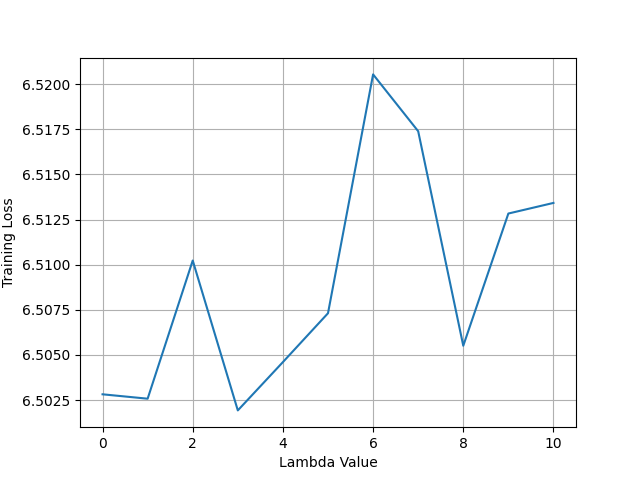
\includegraphics[scale=0.6]{q2.png}
\end{minipage}

\newpage
\textbf{Code for Q2.5)}
\begin{lstlisting}
import numpy as np

def ridgeRegression(x, y, alpha):
    width, height = x.shape
    newX = np.hstack([np.ones((width, 1)), x])

    leftSide = newX.T @ newX + alpha*np.identity(width)
    rightSide = newX.T @ y

    solution = np.linalg.solve(leftSide, rightSide)
    return solution[1:], solution[0]
\end{lstlisting} 
This will give us (w,b) as a result which we can use later on.\\\\
\textbf{Q4)} Below is the algorithm for gradient descent for solving ridge regression, implemented in python:
\begin{lstlisting}
import numpy as np
import pandas as pd;
import matplotlib.pyplot as plt

def ridgeRegression(x, y, alpha):
    width, height = x.shape
    newX = np.hstack([np.ones((width, 1)), x])

    leftSide = newX.T @ newX + alpha * np.identity(height+1)
    rightSide = newX.T @ y

    solution = np.linalg.solve(leftSide, rightSide)
    return solution[1:], solution[0]


def gradiantDescent(x, y, alpha, tolerance, maxiterations, learningRate):
    width, height = x.shape
    b = 0;
    w = np.zeros((height, 1))

    for i in range(0, maxiterations):
        inside = (x @ w + b * np.ones((width, 1)) - y.T)
        deltaw = 1 / width * x.T @ inside + 2 * alpha * w
        deltab = 1 / width * np.ones((1, width)) @ inside

        neww = w + learningRate * deltaw
        newb = b + learningRate * deltab

        if np.linalg.norm(w - neww) < tolerance:
            w = neww
            b = newb
            break
        w = neww
        b = newb

    return w[0], b[0][0]


x = np.array([[1, 1], [2, 2], [3, 3]])

y = np.array([[1, 2, 3]])
w, b = gradiantDescent(x, y, 1, 0.0001, 1, 0.2)

x_test = pd.read_csv("dataset/Housing_X_test.csv", header=None)
x_train = pd.read_csv("dataset/Housing_X_train.csv", header=None)

y_test = pd.read_csv("dataset/Housing_Y_test.csv", header=None)
y_train = pd.read_csv("dataset/Housing_Y_train.csv", header=None)

x_test.fillna(x_test.mean(), inplace=True)
x_train.fillna(x_train.mean(), inplace=True)

# Standardize our data
for i in range(0, 13):
    test = x_test.iloc[i]
    train = x_train.iloc[i]

    minValue = min(test.min(), train.min())
    maxValue = max(test.max(), train.max())

    for idx in range(0, x_train.shape[1]):
        x_train.iloc[i,idx] = (x_train.iloc[i,idx] - minValue)/maxValue
    for idx in range(0, x_test.shape[1]):
        x_test.iloc[i,idx] = (x_test.iloc[i,idx] - minValue)/maxValue

TotalLoss_1 = [0]*11
MSE_1 = [0]*11
TotalLoss_2 = [0]*11
MSE_2 = [0]*11
for h in range(0,11):

    for i in range(0, 9):
        dataToTrainX = np.concatenate([x_train.iloc[:, 0:20*i], x_train.iloc[:,20*(i+1):]], axis=1)
        dataToTrainY = np.concatenate([y_train.iloc[0:20*i], y_train.iloc[20*(i+1):]], axis=0)

        dataToTestY = y_train.iloc[20 * i:20 * (i + 1)]
        dataToTestX = x_train.iloc[:, 20*i:20*(i+1)]
        dataToTestX = dataToTestX.T
        dataToTrainX = dataToTrainX.T

        w1,b1 = ridgeRegression(dataToTrainX, dataToTrainY, 1)
        w2,b2 = gradiantDescent(dataToTrainX,dataToTrainY, 1,       10000, 100000, 0.15)
        for i in range(0,20):
            line = dataToTrainX[i]
            estimate1 = line @ w1 + b1
            estimate2 = line @ w2 + b2
            TotalLoss_1[h] += np.abs(dataToTestY.iloc[i][0] - estimate1)
            TotalLoss_2[h] += np.abs(dataToTestY.iloc[i][0] - estimate2)
            MSE_1[h] += (np.mean(dataToTestY) - estimate1)**2
            MSE_2[h] += (np.mean(dataToTestY) - estimate2) ** 2

    TotalLoss_1[h] = TotalLoss_1[h]/200
    MSE_1[h] = MSE_1[h]/200
    TotalLoss_2[h] = TotalLoss_2[h]/200
    MSE_2[h] = MSE_2[h]/200
    print(h, "loss lin", TotalLoss_1[h])
    print(h, "loss ridge",TotalLoss_2[h])
    print(h, "mse lin train", MSE_1[h])
    print(h, "mse ridge train", MSE_2[h])

    MSE_1[h] = 0
    MSE_2[h] =0

    w1,b1 = ridgeRegression(x_train.T, y_train, 1)
    w2,b2 = gradiantDescent(dataToTrainX,dataToTrainY, 1,       10000, 100000, 0.15)
    for i in range(0, 200):
        line = x_test[i]
        estimate1 = line @ w1 + b1
        estimate2 = line @ w2 + b2
        MSE_1[h] += (np.mean(y_test) - estimate1) ** 2
        MSE_2[h] += (np.mean(y_test) - estimate2) ** 2

    print(h, MSE_1[h]/200)
    print(h, MSE_2[h]/200)

plt.grid(True)
plt.plot([0,1,2,3,4,5,6,7,8,9,10], TotalLoss_2)
plt.title('Lambdas Impact on Training Loss')
plt.xlabel('Lambda Value')
plt.ylabel('Training Loss')
plt.show()
\end{lstlisting} 
\end{titlepage}

\end{document}